% The paper, with its reader's guide.
\part{The Paper}
\chapter*{Reader's guide to the paper}\addcontentsline{toc}{chapter}{Reader's guide to the paper}
The paper follows exactly as published, slightly reduced. Along the foot of each page are the concepts from this book that appear on it, with the chapter that teaches them. The first appearance of each:

\begin{longtable}{p{0.5\textwidth}ll}
Divisibility & Chapter~1 & p.~1 of the paper\\
Even and odd numbers & Chapter~1 & p.~1 of the paper\\
Prime numbers & Chapter~1 & p.~1 of the paper\\
Division with remainder & Chapter~1 & p.~2 of the paper\\
Square numbers & Chapter~1 & p.~2 of the paper\\
\end{longtable}
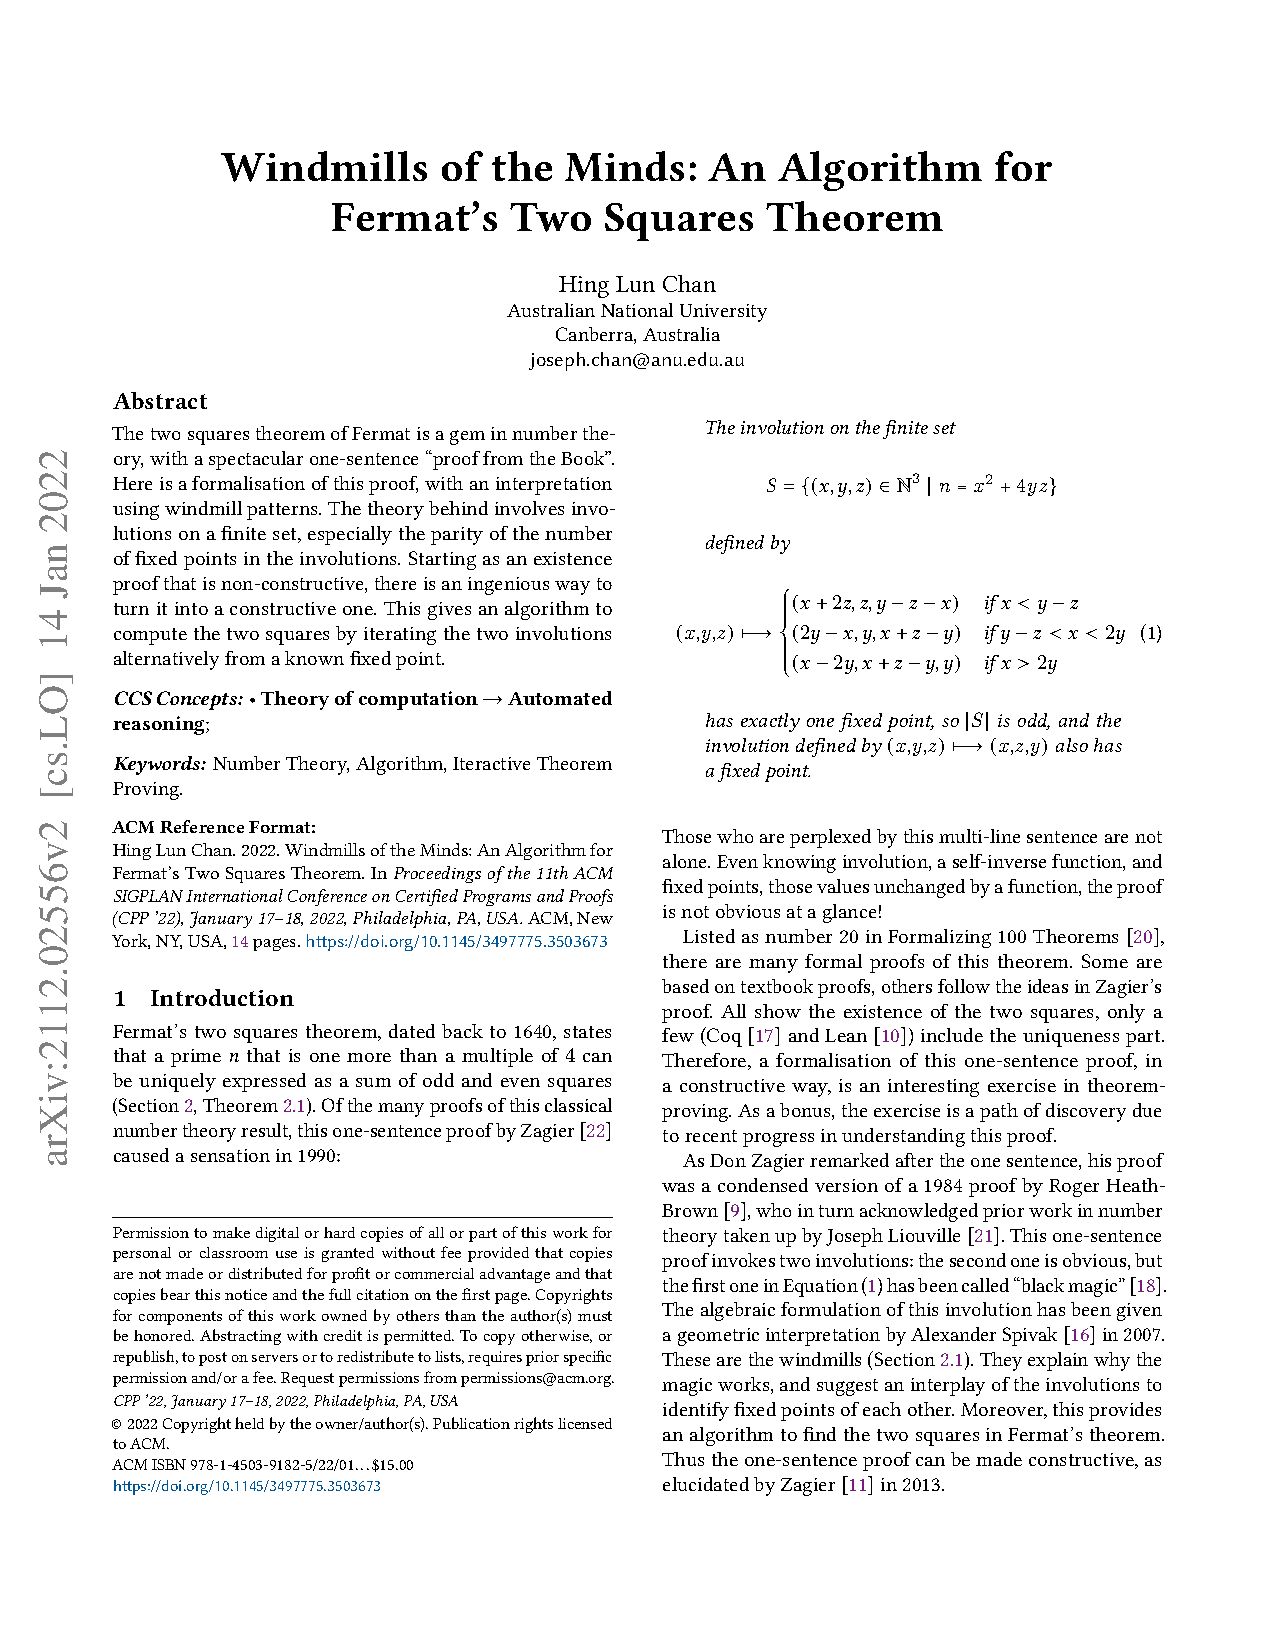
\includepdf[pages=1,scale=0.88,offset=0in 0.42in,pagecommand={\thispagestyle{empty}\papernote{\textbf{In this book:} Divisibility (Ch.~1) \enspace\textperiodcentered\enspace Even and odd numbers (Ch.~1) \enspace\textperiodcentered\enspace Prime numbers (Ch.~1)}}]{paper.pdf}
\includepdf[pages=2,scale=0.88,offset=0in 0.42in,pagecommand={\thispagestyle{empty}\papernote{\textbf{In this book:} Division with remainder (Ch.~1) \enspace\textperiodcentered\enspace Even and odd numbers (Ch.~1) \enspace\textperiodcentered\enspace Prime numbers (Ch.~1) \enspace\textperiodcentered\enspace Square numbers (Ch.~1)}}]{paper.pdf}
\includepdf[pages=3,scale=0.88,offset=0in 0.42in,pagecommand={\thispagestyle{empty}\papernote{\textbf{In this book:} Division with remainder (Ch.~1) \enspace\textperiodcentered\enspace Even and odd numbers (Ch.~1) \enspace\textperiodcentered\enspace Prime numbers (Ch.~1) \enspace\textperiodcentered\enspace Square numbers (Ch.~1)}}]{paper.pdf}
\includepdf[pages=4,scale=0.88,offset=0in 0.42in,pagecommand={\thispagestyle{empty}\papernote{\textbf{In this book:} Prime numbers (Ch.~1) \enspace\textperiodcentered\enspace Square numbers (Ch.~1)}}]{paper.pdf}
\includepdf[pages=5,scale=0.88,offset=0in 0.42in,pagecommand={\thispagestyle{empty}\papernote{}}]{paper.pdf}
\includepdf[pages=6,scale=0.88,offset=0in 0.42in,pagecommand={\thispagestyle{empty}\papernote{}}]{paper.pdf}
\includepdf[pages=7,scale=0.88,offset=0in 0.42in,pagecommand={\thispagestyle{empty}\papernote{\textbf{In this book:} Division with remainder (Ch.~1) \enspace\textperiodcentered\enspace Even and odd numbers (Ch.~1) \enspace\textperiodcentered\enspace Prime numbers (Ch.~1) \enspace\textperiodcentered\enspace Square numbers (Ch.~1)}}]{paper.pdf}
\includepdf[pages=8,scale=0.88,offset=0in 0.42in,pagecommand={\thispagestyle{empty}\papernote{}}]{paper.pdf}
\includepdf[pages=9,scale=0.88,offset=0in 0.42in,pagecommand={\thispagestyle{empty}\papernote{\textbf{In this book:} Divisibility (Ch.~1) \enspace\textperiodcentered\enspace Division with remainder (Ch.~1) \enspace\textperiodcentered\enspace Even and odd numbers (Ch.~1)}}]{paper.pdf}
\includepdf[pages=10,scale=0.88,offset=0in 0.42in,pagecommand={\thispagestyle{empty}\papernote{\textbf{In this book:} Divisibility (Ch.~1) \enspace\textperiodcentered\enspace Division with remainder (Ch.~1) \enspace\textperiodcentered\enspace Even and odd numbers (Ch.~1)}}]{paper.pdf}
\includepdf[pages=11,scale=0.88,offset=0in 0.42in,pagecommand={\thispagestyle{empty}\papernote{\textbf{In this book:} Division with remainder (Ch.~1) \enspace\textperiodcentered\enspace Even and odd numbers (Ch.~1) \enspace\textperiodcentered\enspace Prime numbers (Ch.~1)}}]{paper.pdf}
\includepdf[pages=12,scale=0.88,offset=0in 0.42in,pagecommand={\thispagestyle{empty}\papernote{\textbf{In this book:} Division with remainder (Ch.~1) \enspace\textperiodcentered\enspace Even and odd numbers (Ch.~1) \enspace\textperiodcentered\enspace Prime numbers (Ch.~1) \enspace\textperiodcentered\enspace Square numbers (Ch.~1)}}]{paper.pdf}
\includepdf[pages=13,scale=0.88,offset=0in 0.42in,pagecommand={\thispagestyle{empty}\papernote{\textbf{In this book:} Prime numbers (Ch.~1)}}]{paper.pdf}
\includepdf[pages=14,scale=0.88,offset=0in 0.42in,pagecommand={\thispagestyle{empty}\papernote{\textbf{In this book:} Division with remainder (Ch.~1) \enspace\textperiodcentered\enspace Prime numbers (Ch.~1) \enspace\textperiodcentered\enspace Square numbers (Ch.~1)}}]{paper.pdf}